\documentclass{article}
\usepackage{ifthen}
\usepackage{amssymb}
\usepackage{multicol}
\usepackage{graphicx}
\usepackage[absolute]{textpos}
\usepackage{amsmath, amscd, amssymb, amsthm, latexsym}
% \usepackage[noload]{qtree}
%\usepackage{xspace,rotating,calligra,dsfont,ifthen}
\usepackage{xspace,rotating,dsfont,ifthen}
\usepackage[spanish,activeacute]{babel}
\usepackage[utf8]{inputenc}
\usepackage{pgfpages}
\usepackage{pgf,pgfarrows,pgfnodes,pgfautomata,pgfheaps,xspace,dsfont}
\usepackage{listings}
\usepackage{multicol}
\usepackage{todonotes}
\usepackage{url}
\usepackage{float}
\usepackage{framed,mdframed}
\usepackage{cancel}

\usepackage[strict]{changepage}


\makeatletter


\newcommand\hfrac[2]{\genfrac{}{}{0pt}{}{#1}{#2}} %\hfrac{}{} es un \frac sin la linea del medio

\newcommand\Wider[2][3em]{% \Wider[3em]{} reduce los m\'argenes
\makebox[\linewidth][c]{%
  \begin{minipage}{\dimexpr\textwidth+#1\relax}
  \raggedright#2
  \end{minipage}%
  }%
}


\@ifclassloaded{beamer}{%
  \newcommand{\tocarEspacios}{%
    \addtolength{\leftskip}{4em}%
    \addtolength{\parindent}{-3em}%
  }%
}
{%
  \usepackage[top=1cm,bottom=2cm,left=1cm,right=1cm]{geometry}%
  \usepackage{color}%
  \newcommand{\tocarEspacios}{%
    \addtolength{\leftskip}{3em}%
    \setlength{\parindent}{0em}%
  }%
}

\newcommand{\encabezadoDeProc}[4]{%
  % Ponemos la palabrita problema en tt
%  \noindent%
  {\normalfont\bfseries\ttfamily proc}%
  % Ponemos el nombre del problema
  \ %
  {\normalfont\ttfamily #2}%
  \
  % Ponemos los parametros
  (#3)%
  \ifthenelse{\equal{#4}{}}{}{%
  \ =\ %
  % Ponemos el nombre del resultado
  {\normalfont\ttfamily #1}%
  % Por ultimo, va el tipo del resultado
  \ : #4}
}

\newcommand{\encabezadoDeTipo}[2]{%
  % Ponemos la palabrita tipo en tt
  {\normalfont\bfseries\ttfamily tipo}%
  % Ponemos el nombre del tipo
  \ %
  {\normalfont\ttfamily #2}%
  \ifthenelse{\equal{#1}{}}{}{$\langle$#1$\rangle$}
}

% Primero definiciones de cosas al estilo title, author, date

\def\materia#1{\gdef\@materia{#1}}
\def\@materia{No especifi\'o la materia}
\def\lamateria{\@materia}

\def\cuatrimestre#1{\gdef\@cuatrimestre{#1}}
\def\@cuatrimestre{No especifi\'o el cuatrimestre}
\def\elcuatrimestre{\@cuatrimestre}

\def\anio#1{\gdef\@anio{#1}}
\def\@anio{No especifi\'o el anio}
\def\elanio{\@anio}

\def\fecha#1{\gdef\@fecha{#1}}
\def\@fecha{\today}
\def\lafecha{\@fecha}

\def\nombre#1{\gdef\@nombre{#1}}
\def\@nombre{No especific'o el nombre}
\def\elnombre{\@nombre}

\def\practicas#1{\gdef\@practica{#1}}
\def\@practica{No especifi\'o el n\'umero de pr\'actica}
\def\lapractica{\@practica}


% Esta macro convierte el numero de cuatrimestre a palabras
\newcommand{\cuatrimestreLindo}{
  \ifthenelse{\equal{\elcuatrimestre}{1}}
  {Primer cuatrimestre}
  {\ifthenelse{\equal{\elcuatrimestre}{2}}
  {Segundo cuatrimestre}
  {Verano}}
}


\newcommand{\depto}{{UBA -- Facultad de Ciencias Exactas y Naturales --
      Departamento de Computaci\'on}}

\newcommand{\titulopractica}{
  \centerline{\depto}
  \vspace{1ex}
  \centerline{{\Large\lamateria}}
  \vspace{0.5ex}
  \centerline{\cuatrimestreLindo de \elanio}
  \vspace{2ex}
  \centerline{{\huge Pr\'actica \lapractica -- \elnombre}}
  \vspace{5ex}
  \arreglarincisos
  \newcounter{ejercicio}
  \newenvironment{ejercicio}{\stepcounter{ejercicio}\textbf{Ejercicio
      \theejercicio}%
    \renewcommand\@currentlabel{\theejercicio}%
  }{\vspace{0.2cm}}
}


\newcommand{\titulotp}{
  \centerline{\depto}
  \vspace{1ex}
  \centerline{{\Large\lamateria}}
  \vspace{0.5ex}
  \centerline{\cuatrimestreLindo de \elanio}
  \vspace{0.5ex}
  \centerline{\lafecha}
  \vspace{2ex}
  \centerline{{\huge\elnombre}}
  \vspace{5ex}
}


%practicas
\newcommand{\practica}[2]{%
    \title{Pr\'actica #1 \\ #2}
    \author{Algoritmos y Estructuras de Datos I}
    \date{Segundo Cuatrimestre 2019}

    \maketitlepractica{#1}{#2}
}

\newcommand \maketitlepractica[2] {%
\begin{center}
\begin{tabular}{r cr}
 \begin{tabular}{c}
{\large\bf\textsf{\ Algoritmos y Estructuras de Datos I\ }}\\
Primer Cuatrimestre 2021\\
\title{\normalsize Gu\'ia Pr\'actica #1 \\ \textbf{#2}}\\
\@title
\end{tabular} &
\begin{tabular}{@{} p{1.6cm} @{}}
\includegraphics[width=1.6cm]{logodpt.jpg}
\end{tabular} &
\begin{tabular}{l @{}}
 \emph{Departamento de Computaci\'on} \\
 \emph{Facultad de Ciencias Exactas y Naturales} \\
 \emph{Universidad de Buenos Aires} \\
\end{tabular}
\end{tabular}
\end{center}

\bigskip
}


% Símbolos varios

\newcommand{\nat}{\ensuremath{\mathds{N}}}
\newcommand{\ent}{\ensuremath{\mathds{Z}}}
\newcommand{\float}{\ensuremath{\mathds{R}}}
\newcommand{\bool}{\ensuremath{\mathsf{Bool}}}
\newcommand{\True}{\ensuremath{\mathrm{true}}}
\newcommand{\False}{\ensuremath{\mathrm{false}}}
\newcommand{\Then}{\ensuremath{\rightarrow}}
\newcommand{\Iff}{\ensuremath{\leftrightarrow}}
\newcommand{\implica}{\ensuremath{\longrightarrow}}
\newcommand{\IfThenElse}[3]{\ensuremath{\mathsf{if}\ #1\ \mathsf{then}\ #2\ \mathsf{else}\ #3\ \mathsf{fi}}}
\newcommand{\In}{\textsf{in }}
\newcommand{\Out}{\textsf{out }}
\newcommand{\Inout}{\textsf{inout }}
\newcommand{\yLuego}{\land _L}
\newcommand{\oLuego}{\lor _L}
\newcommand{\implicaLuego}{\implica _L}
\newcommand{\cuantificador}[5]{%
	\ensuremath{(#2 #3: #4)\ (%
		\ifthenelse{\equal{#1}{unalinea}}{
			#5
		}{
			$ % exiting math mode
			\begin{adjustwidth}{+2em}{}
			$#5$%
			\end{adjustwidth}%
			$ % entering math mode
		}
	)}
}

\newcommand{\existe}[4][]{%
	\cuantificador{#1}{\exists}{#2}{#3}{#4}
}
\newcommand{\paraTodo}[4][]{%
	\cuantificador{#1}{\forall}{#2}{#3}{#4}
}

% Símbolo para marcar los ejercicios importantes (estrellita)
\newcommand\importante{\raisebox{0.5pt}{\ensuremath{\bigstar}}}


\newcommand{\rango}[2]{[#1\twodots#2]}
\newcommand{\comp}[2]{[\,#1\,|\,#2\,]}

\newcommand{\rangoac}[2]{(#1\twodots#2]}
\newcommand{\rangoca}[2]{[#1\twodots#2)}
\newcommand{\rangoaa}[2]{(#1\twodots#2)}

%ejercicios
\newtheorem{exercise}{Ejercicio}
\newenvironment{ejercicio}[1][]{\begin{exercise}#1\rm}{\end{exercise} \vspace{0.2cm}}
\newenvironment{items}{\begin{enumerate}[a)]}{\end{enumerate}}
\newenvironment{subitems}{\begin{enumerate}[i)]}{\end{enumerate}}
\newcommand{\sugerencia}[1]{\noindent \textbf{Sugerencia:} #1}

\lstnewenvironment{code}{
    \lstset{% general command to set parameter(s)
        language=C++, basicstyle=\small\ttfamily, keywordstyle=\slshape,
        emph=[1]{tipo,usa}, emphstyle={[1]\sffamily\bfseries},
        morekeywords={tint,forn,forsn},
        basewidth={0.47em,0.40em},
        columns=fixed, fontadjust, resetmargins, xrightmargin=5pt, xleftmargin=15pt,
        flexiblecolumns=false, tabsize=2, breaklines, breakatwhitespace=false, extendedchars=true,
        numbers=left, numberstyle=\tiny, stepnumber=1, numbersep=9pt,
        frame=l, framesep=3pt,
    }
   \csname lst@SetFirstLabel\endcsname}
  {\csname lst@SaveFirstLabel\endcsname}


%tipos basicos
\newcommand{\rea}{\ensuremath{\mathsf{Float}}}
\newcommand{\cha}{\ensuremath{\mathsf{Char}}}
\newcommand{\str}{\ensuremath{\mathsf{String}}}

\newcommand{\mcd}{\mathrm{mcd}}
\newcommand{\prm}[1]{\ensuremath{\mathsf{prm}(#1)}}
\newcommand{\sgd}[1]{\ensuremath{\mathsf{sgd}(#1)}}

\newcommand{\tuple}[2]{\ensuremath{#1 \times #2}}

%listas
\newcommand{\TLista}[1]{\ensuremath{seq \langle #1\rangle}}
\newcommand{\lvacia}{\ensuremath{[\ ]}}
\newcommand{\lv}{\ensuremath{[\ ]}}
\newcommand{\longitud}[1]{\ensuremath{|#1|}}
\newcommand{\cons}[1]{\ensuremath{\mathsf{addFirst}}(#1)}
\newcommand{\indice}[1]{\ensuremath{\mathsf{indice}}(#1)}
\newcommand{\conc}[1]{\ensuremath{\mathsf{concat}}(#1)}
\newcommand{\cab}[1]{\ensuremath{\mathsf{head}}(#1)}
\newcommand{\cola}[1]{\ensuremath{\mathsf{tail}}(#1)}
\newcommand{\sub}[1]{\ensuremath{\mathsf{subseq}}(#1)}
\newcommand{\en}[1]{\ensuremath{\mathsf{en}}(#1)}
\newcommand{\cuenta}[2]{\mathsf{cuenta}\ensuremath{(#1, #2)}}
\newcommand{\suma}[1]{\mathsf{suma}(#1)}
\newcommand{\twodots}{\ensuremath{\mathrm{..}}}
\newcommand{\masmas}{\ensuremath{++}}
\newcommand{\matriz}[1]{\TLista{\TLista{#1}}}

\newcommand{\seqchar}{\TLista{\cha}}


% Acumulador
\newcommand{\acum}[1]{\ensuremath{\mathsf{acum}}(#1)}
\newcommand{\acumselec}[3]{\ensuremath{\mathrm{acum}(#1 |  #2, #3)}}

% \selector{variable}{dominio}
\newcommand{\selector}[2]{#1~\ensuremath{\leftarrow}~#2}
\newcommand{\selec}{\ensuremath{\leftarrow}}

\newcommand{\pred}[3]{%
    {\normalfont\bfseries\ttfamily\noindent pred }%
    {\normalfont\ttfamily #1}%
    \ifthenelse{\equal{#2}{}}{}{\ (#2) }%
    \{%
    \begin{adjustwidth}{+2em}{}
      \ensuremath{#3}
    \end{adjustwidth}
    \}%
    {\normalfont\bfseries\,\par}%
}

\newenvironment{proc}[4][res]{%

  % El parametro 1 (opcional) es el nombre del resultado
  % El parametro 2 es el nombre del problema
  % El parametro 3 son los parametros
  % El parametro 4 es el tipo del resultado
  % Preambulo del ambiente problema
  % Tenemos que definir los comandos requiere, asegura, modifica y aux
  \newcommand{\pre}[2][]{%
    {\normalfont\bfseries\ttfamily Pre}%
    \ifthenelse{\equal{##1}{}}{}{\ {\normalfont\ttfamily ##1} :}\ %
    \{\ensuremath{##2}\}%
    {\normalfont\bfseries\,\par}%
  }
  \newcommand{\post}[2][]{%
    {\normalfont\bfseries\ttfamily Post}%
    \ifthenelse{\equal{##1}{}}{}{\ {\normalfont\ttfamily ##1} :}\
    \{\ensuremath{##2}\}%
    {\normalfont\bfseries\,\par}%
  }
  \renewcommand{\aux}[4]{%
    {\normalfont\bfseries\ttfamily aux\ }%
    {\normalfont\ttfamily ##1}%
    \ifthenelse{\equal{##2}{}}{}{\ (##2)}\ : ##3\, = \ensuremath{##4}%
    {\normalfont\bfseries\,;\par}%
  }
  \renewcommand{\pred}[3]{%
    {\normalfont\bfseries\ttfamily pred }%
    {\normalfont\ttfamily ##1}%
    \ifthenelse{\equal{##2}{}}{}{\ (##2) }%
    \{%
    \begin{adjustwidth}{+5em}{}
      \ensuremath{##3}
    \end{adjustwidth}
    \}%
    {\normalfont\bfseries\,\par}%
  }

  \newcommand{\res}{#1}
  \vspace{1ex}
  \noindent
  \encabezadoDeProc{#1}{#2}{#3}{#4}
  % Abrimos la llave
  \{\par%
  \tocarEspacios
}
% Ahora viene el cierre del ambiente problema
{
  % Cerramos la llave
  \noindent\}
  \vspace{1ex}
}


\newcommand{\aux}[4]{%
    {\normalfont\bfseries\ttfamily\noindent aux\ }%
    {\normalfont\ttfamily #1}%
    \ifthenelse{\equal{#2}{}}{}{\ (#2)}\ : #3\, = \ensuremath{#4}%
    {\normalfont\bfseries\,;\par}%
}


% \newcommand{\pre}[1]{\textsf{pre}\ensuremath{(#1)}}

\newcommand{\procnom}[1]{\textsf{#1}}
\newcommand{\procil}[3]{\textsf{proc #1}\ensuremath{(#2) = #3}}
\newcommand{\procilsinres}[2]{\textsf{proc #1}\ensuremath{(#2)}}
\newcommand{\preil}[2]{\textsf{Pre #1: }\ensuremath{#2}}
\newcommand{\postil}[2]{\textsf{Post #1: }\ensuremath{#2}}
\newcommand{\auxil}[2]{\textsf{fun }\ensuremath{#1 = #2}}
\newcommand{\auxilc}[4]{\textsf{fun }\ensuremath{#1( #2 ): #3 = #4}}
\newcommand{\auxnom}[1]{\textsf{fun }\ensuremath{#1}}
\newcommand{\auxpred}[3]{\textsf{pred }\ensuremath{#1( #2 ) \{ #3 \}}}

\newcommand{\comentario}[1]{{/*\ #1\ */}}

\newcommand{\nom}[1]{\ensuremath{\mathsf{#1}}}


% En las practicas/parciales usamos numeros arabigos para los ejercicios.
% Aca cambiamos los enumerate comunes para que usen letras y numeros
% romanos
\newcommand{\arreglarincisos}{%
  \renewcommand{\theenumi}{\alph{enumi}}
  \renewcommand{\theenumii}{\roman{enumii}}
  \renewcommand{\labelenumi}{\theenumi)}
  \renewcommand{\labelenumii}{\theenumii)}
}



%%%%%%%%%%%%%%%%%%%%%%%%%%%%%% PARCIAL %%%%%%%%%%%%%%%%%%%%%%%%
\let\@xa\expandafter
\newcommand{\tituloparcial}{\centerline{\depto -- \lamateria}
  \centerline{\elnombre -- \lafecha}%
  \setlength{\TPHorizModule}{10mm} % Fija las unidades de textpos
  \setlength{\TPVertModule}{\TPHorizModule} % Fija las unidades de
                                % textpos
  \arreglarincisos
  \newcounter{total}% Este contador va a guardar cuantos incisos hay
                    % en el parcial. Si un ejercicio no tiene incisos,
                    % cuenta como un inciso.
  \newcounter{contgrilla} % Para hacer ciclos
  \newcounter{columnainicial} % Se van a usar para los cline cuando un
  \newcounter{columnafinal}   % ejercicio tenga incisos.
  \newcommand{\primerafila}{}
  \newcommand{\segundafila}{}
  \newcommand{\rayitas}{} % Esto va a guardar los \cline de los
                          % ejercicios con incisos, asi queda mas bonito
  \newcommand{\anchodegrilla}{20} % Es para textpos
  \newcommand{\izquierda}{7} % Estos dos le dicen a textpos donde colocar
  \newcommand{\abajo}{2}     % la grilla
  \newcommand{\anchodecasilla}{0.4cm}
  \setcounter{columnainicial}{1}
  \setcounter{total}{0}
  \newcounter{ejercicio}
  \setcounter{ejercicio}{0}
  \renewenvironment{ejercicio}[1]
  {%
    \stepcounter{ejercicio}\textbf{\noindent Ejercicio \theejercicio. [##1
      puntos]}% Formato
    \renewcommand\@currentlabel{\theejercicio}% Esto es para las
                                % referencias
    \newcommand{\invariante}[2]{%
      {\normalfont\bfseries\ttfamily invariante}%
      \ ####1\hspace{1em}####2%
    }%
    \newcommand{\Proc}[5][result]{
      \encabezadoDeProc{####1}{####2}{####3}{####4}\hspace{1em}####5}%
  }% Aca se termina el principio del ejercicio
  {% Ahora viene el final
    % Esto suma la cantidad de incisos o 1 si no hubo ninguno
    \ifthenelse{\equal{\value{enumi}}{0}}
    {\addtocounter{total}{1}}
    {\addtocounter{total}{\value{enumi}}}
    \ifthenelse{\equal{\value{ejercicio}}{1}}{}
    {
      \g@addto@macro\primerafila{&} % Si no estoy en el primer ej.
      \g@addto@macro\segundafila{&}
    }
    \ifthenelse{\equal{\value{enumi}}{0}}
    {% No tiene incisos
      \g@addto@macro\primerafila{\multicolumn{1}{|c|}}
      \bgroup% avoid overwriting somebody else's value of \tmp@a
      \protected@edef\tmp@a{\theejercicio}% expand as far as we can
      \@xa\g@addto@macro\@xa\primerafila\@xa{\tmp@a}%
      \egroup% restore old value of \tmp@a, effect of \g@addto.. is

      \stepcounter{columnainicial}
    }
    {% Tiene incisos
      % Primero ponemos el encabezado
      \g@addto@macro\primerafila{\multicolumn}% Ahora el numero de items
      \bgroup% avoid overwriting somebody else's value of \tmp@a
      \protected@edef\tmp@a{\arabic{enumi}}% expand as far as we can
      \@xa\g@addto@macro\@xa\primerafila\@xa{\tmp@a}%
      \egroup% restore old value of \tmp@a, effect of \g@addto.. is
      % global
      % Ahora el formato
      \g@addto@macro\primerafila{{|c|}}%
      % Ahora el numero de ejercicio
      \bgroup% avoid overwriting somebody else's value of \tmp@a
      \protected@edef\tmp@a{\theejercicio}% expand as far as we can
      \@xa\g@addto@macro\@xa\primerafila\@xa{\tmp@a}%
      \egroup% restore old value of \tmp@a, effect of \g@addto.. is
      % global
      % Ahora armamos la segunda fila
      \g@addto@macro\segundafila{\multicolumn{1}{|c|}{a}}%
      \setcounter{contgrilla}{1}
      \whiledo{\value{contgrilla}<\value{enumi}}
      {%
        \stepcounter{contgrilla}
        \g@addto@macro\segundafila{&\multicolumn{1}{|c|}}
        \bgroup% avoid overwriting somebody else's value of \tmp@a
        \protected@edef\tmp@a{\alph{contgrilla}}% expand as far as we can
        \@xa\g@addto@macro\@xa\segundafila\@xa{\tmp@a}%
        \egroup% restore old value of \tmp@a, effect of \g@addto.. is
        % global
      }
      % Ahora armo las rayitas
      \setcounter{columnafinal}{\value{columnainicial}}
      \addtocounter{columnafinal}{-1}
      \addtocounter{columnafinal}{\value{enumi}}
      \bgroup% avoid overwriting somebody else's value of \tmp@a
      \protected@edef\tmp@a{\noexpand\cline{%
          \thecolumnainicial-\thecolumnafinal}}%
      \@xa\g@addto@macro\@xa\rayitas\@xa{\tmp@a}%
      \egroup% restore old value of \tmp@a, effect of \g@addto.. is
      \setcounter{columnainicial}{\value{columnafinal}}
      \stepcounter{columnainicial}
    }
    \setcounter{enumi}{0}%
    \vspace{0.2cm}%
  }%
  \newcommand{\tercerafila}{}
  \newcommand{\armartercerafila}{
    \setcounter{contgrilla}{1}
    \whiledo{\value{contgrilla}<\value{total}}
    {\stepcounter{contgrilla}\g@addto@macro\tercerafila{&}}
  }
  \newcommand{\grilla}{%
    \g@addto@macro\primerafila{&\textbf{TOTAL}}
    \g@addto@macro\segundafila{&}
    \g@addto@macro\tercerafila{&}
    \armartercerafila
    \ifthenelse{\equal{\value{total}}{\value{ejercicio}}}
    {% No hubo incisos
      \begin{textblock}{\anchodegrilla}(\izquierda,\abajo)
        \begin{tabular}{|*{\value{total}}{p{\anchodecasilla}|}c|}
          \hline
          \primerafila\\
          \hline
          \tercerafila\\
          \tercerafila\\
          \hline
        \end{tabular}
      \end{textblock}
    }
    {% Hubo incisos
      \begin{textblock}{\anchodegrilla}(\izquierda,\abajo)
        \begin{tabular}{|*{\value{total}}{p{\anchodecasilla}|}c|}
          \hline
          \primerafila\\
          \rayitas
          \segundafila\\
          \hline
          \tercerafila\\
          \tercerafila\\
          \hline
        \end{tabular}
      \end{textblock}
    }
  }%
  % \datosalumno
}

\newcommand{\datosalumno}{
  \vspace{0.4cm}
  \textbf{Apellidos:}

  \textbf{Nombres:}

  \textbf{LU:}

  \textbf{Correo electrónico:}

  \textbf{Nro. de carillas que adjunta:}
  \vspace{0.5cm}
}


% AMBIENTE CONSIGNAS
% Se usa en el TP para ir agregando las cosas que tienen que resolver
% los alumnos.
% Dentro del ambiente hay que usar \item para cada consigna

\newcounter{consigna}
\setcounter{consigna}{0}

\newenvironment{consignas}{%
  \newcommand{\consigna}{\stepcounter{consigna}\textbf{\theconsigna.}}%
  \renewcommand{\ejercicio}[1]{\item ##1 }
  \renewcommand{\proc}[5][result]{\item
    \encabezadoDeProc{##1}{##2}{##3}{##4}\hspace{1em}##5}%
  \newcommand{\invariante}[2]{\item%
    {\normalfont\bfseries\ttfamily invariante}%
    \ ##1\hspace{1em}##2%
  }
  \renewcommand{\aux}[4]{\item%
    {\normalfont\bfseries\ttfamily aux\ }%
    {\normalfont\ttfamily ##1}%
    \ifthenelse{\equal{##2}{}}{}{\ (##2)}\ : ##3 \hspace{1em}##4%
  }
  % Comienza la lista de consignas
  \begin{list}{\consigna}{%
      \setlength{\itemsep}{0.5em}%
      \setlength{\parsep}{0cm}%
    }
}%
{\end{list}}



% para decidir si usar && o ^
\newcommand{\y}[0]{\ensuremath{\land}}

% macros de correctitud
\newcommand{\semanticComment}[2]{#1 \ensuremath{#2};}
\newcommand{\namedSemanticComment}[3]{#1 #2: \ensuremath{#3};}


\newcommand{\local}[1]{\semanticComment{local}{#1}}

\newcommand{\vale}[1]{\semanticComment{vale}{#1}}
\newcommand{\valeN}[2]{\namedSemanticComment{vale}{#1}{#2}}
\newcommand{\impl}[1]{\semanticComment{implica}{#1}}
\newcommand{\implN}[2]{\namedSemanticComment{implica}{#1}{#2}}
\newcommand{\estado}[1]{\semanticComment{estado}{#1}}

\newcommand{\invarianteCN}[2]{\namedSemanticComment{invariante}{#1}{#2}}
\newcommand{\invarianteC}[1]{\semanticComment{invariante}{#1}}
\newcommand{\varianteCN}[2]{\namedSemanticComment{variante}{#1}{#2}}
\newcommand{\varianteC}[1]{\semanticComment{variante}{#1}}
\usepackage{caratula}
\usepackage{enumerate}
\usepackage{hyperref}
\usepackage{graphicx}
\usepackage{amsfonts}
\usepackage{enumitem}

\decimalpoint
\hypersetup{colorlinks=true, linkcolor=black, urlcolor=blue}
\setlength{\parindent}{0em}
\setlength{\parskip}{0.5em}
\setcounter{tocdepth}{2} % profundidad de indice
\setcounter{section}{5} % nro de práctica - 1
\renewcommand{\thesubsubsection}{\thesubsection.\Alph{subsubsection}}
\graphicspath{ {images/} }

% End latex config

\begin{document}

\titulo{Práctica 6}
\fecha{1er cuatrimestre 2022 }
\materia{Algoritmos y Estructuras de Datos 1}
\integrante{Yago Pajariño}{546/21}{ypajarino@dc.uba.ar}

%Carátula
\maketitle
\newpage

%Indice
\tableofcontents
\newpage

% Aca empieza lo propio del documento
\section{Práctica 6}

\subsection{Ejercicio 1}
\subsubsection{Pregunta i}
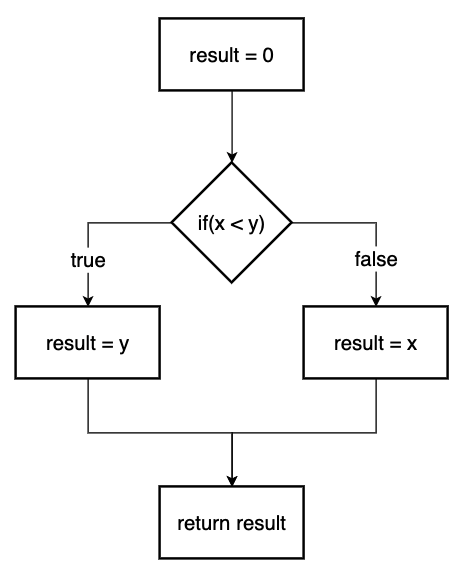
\includegraphics[width=200px]{6.1.1}

\subsubsection{Pregunta ii}
\begin{tabular}{|l|l|l|l|l|l|} 
    \hline
    Test  & L1 & L2 & L3 & L4 & L5  \\ 
    \hline
    test1 & X  & X  &    & X  & X   \\ 
    \hline
    test2 & X  & X  & X  &    & X   \\
    \hline
\end{tabular}

\subsubsection{Pregunta iii}
\begin{tabular}{|l|l|l|} 
    \hline
    Test  & L2-true & L2-false  \\ 
    \hline
    test1 &         & X         \\ 
    \hline
    test2 & X       &           \\
    \hline
\end{tabular}

\subsubsection{Pregunta iv}
Es verdadera.

\subsection{Ejercicio 2}
\subsubsection{Pregunta i}
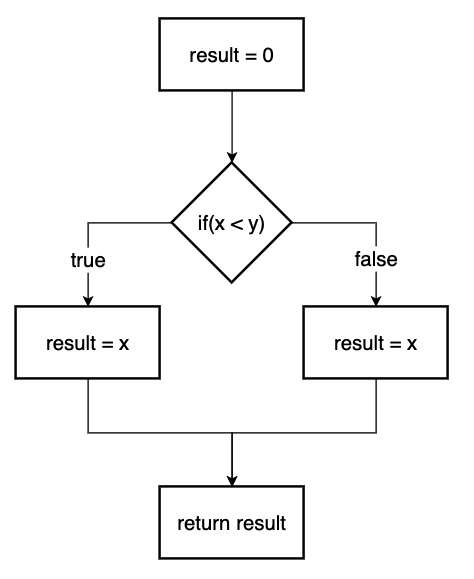
\includegraphics[width=200px]{6.2.1}

\subsubsection{Pregunta ii}
Sí

\subsubsection{Pregunta iii}
Sí

\subsubsection{Pregunta iv}
Sí

\subsubsection{Pregunta v}
No es necesario, ya que el primer test detecta el error, al devolver 1 en lugar de 0 como se esperaba

\subsection{Ejercicio 3}
\subsubsection{Pregunta i}
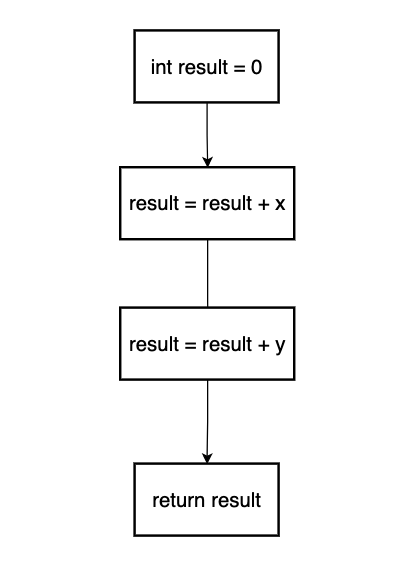
\includegraphics[width=200px]{6.3.1}

\subsubsection{Pregunta ii}
Se ve que cualquier test corre todas las lineas del programa, por lo que:

test1:
\begin{itemize}
    \item Entrada. $ x = 1 $, $ y = 1 $
    \item Salida esperada $ 2 $
\end{itemize}

\subsection{Ejercicio 4}
\subsubsection{Pregunta i}
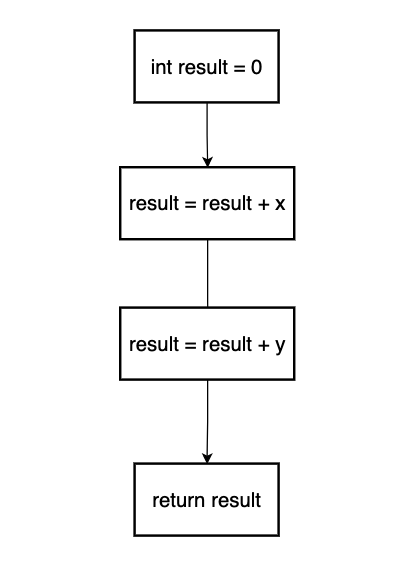
\includegraphics[width=200px]{6.3.1}

\subsubsection{Pregunta ii}
Al igual que en ejercicio anterior, cualquier test ejecuta todas las lineas.

test1:
\begin{itemize}
    \item Entrada. $ x = 1 $, $ y = 1 $
    \item Salida esperada $ 0 $
\end{itemize}

\subsubsection{Pregunta iii}
Sí, lo detecta ya que la salida esperada es 0 pero la implementación devuelve 2.

\subsection{Ejercicio 5}
\subsubsection{Pregunta i}
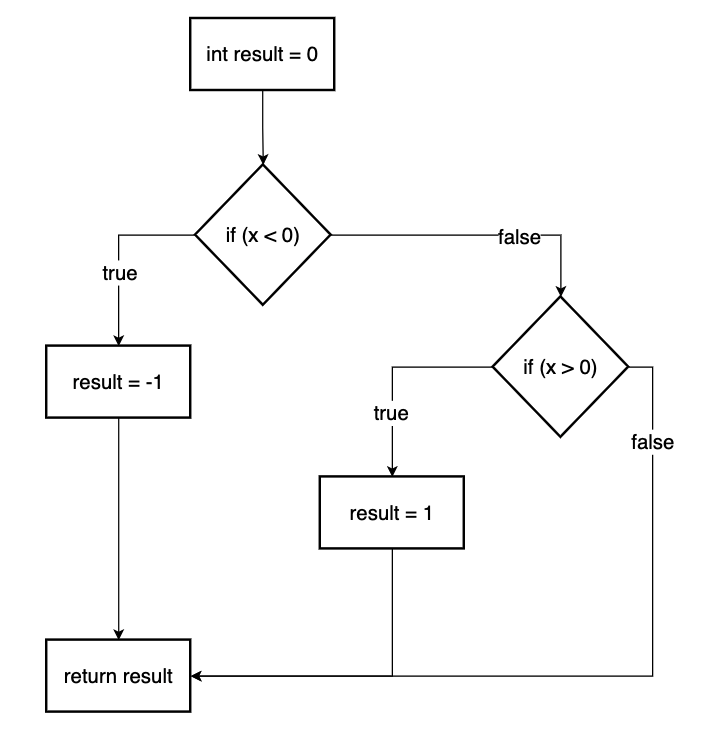
\includegraphics[width=300px]{6.5.1}

\subsubsection{Pregunta ii}
test1:
\begin{itemize}
    \item Entrada. $ x = -1 $
    \item Salida esperada $ -1 $
\end{itemize}

test2:
\begin{itemize}
    \item Entrada. $ x = 1 $
    \item Salida esperada $ 1 $
\end{itemize}

El test suite formado por test1, test2 sjecuta todas las lineas del programa.

\subsubsection{Pregunta iii}
No ejecuta todas las ramas del programa pues faltaría el caso de $x = 0$

\subsection{Ejercicio 6}
\subsubsection{Pregunta i}
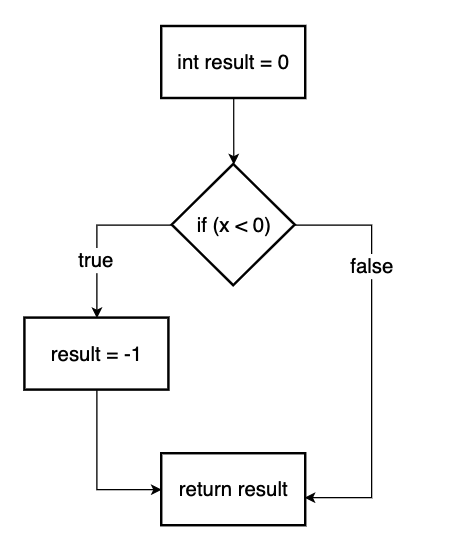
\includegraphics[width=250px]{6.6.1}

\subsubsection{Pregunta ii}
test1:
\begin{itemize}
    \item Entrada. $ x = -1 $
    \item Salida esperada $ -1 $
\end{itemize}

\subsubsection{Pregunta iii}
test1:
\begin{itemize}
    \item Entrada. $ x = -1 $
    \item Salida esperada $ -1 $
\end{itemize}

test2:
\begin{itemize}
    \item Entrada. $ x = 1 $
    \item Salida esperada $ 1 $
\end{itemize}

\subsubsection{Pregunta iv}
test1:
\begin{itemize}
    \item Entrada. $ x = -1 $
    \item Salida esperada $ -1 $
\end{itemize}

\subsection{Ejercicio 7}
\subsubsection{Pregunta i}
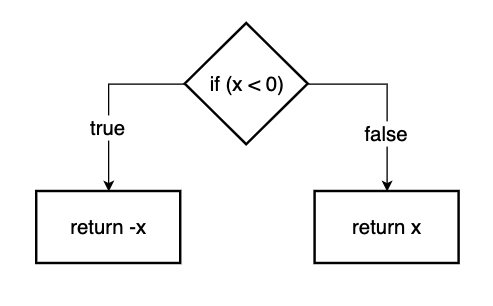
\includegraphics[width=250px]{6.7.1}

\subsubsection{Pregunta ii}
test1 "negativo":
\begin{itemize}
    \item Entrada. $ x = -1 $
    \item Salida esperada. $ 1 $
\end{itemize}

test1 "positivo":
\begin{itemize}
    \item Entrada. $ x = 1 $
    \item Salida esperada. $ 1 $
\end{itemize}

El test suite (test1, test2) cubre todas las líneas y branches del programa.

\subsection{Ejercicio 8}
\subsubsection{Pregunta i}
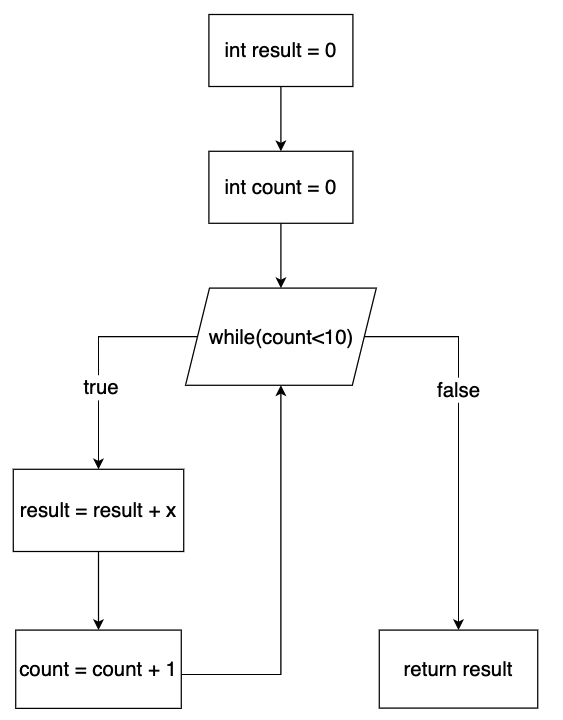
\includegraphics[width=250px]{6.8.1}

\subsubsection{Pregunta ii}
test1:
\begin{itemize}
    \item Entrada. $ x = 5 $
    \item Salida esperada. $ 50 $
\end{itemize}

\subsubsection{Pregunta iii}
Sí

\subsection{Ejercicio 9}
\subsubsection{Pregunta i}
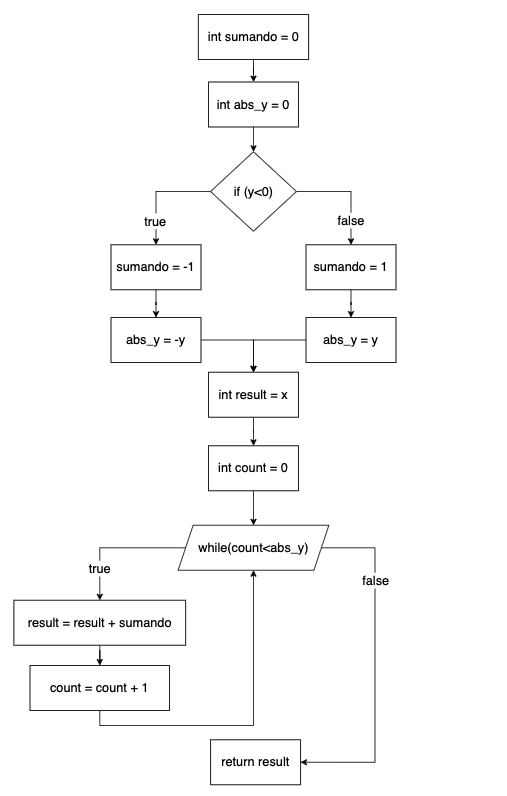
\includegraphics[width=300px]{6.9.1}

\subsubsection{Pregunta ii}
test1 'y positivo':
\begin{itemize}
    \item Entrada. $ x = 1, y = 5 $
    \item Salida esperada. $ 6 $
\end{itemize}

test2 'y negativo':
\begin{itemize}
    \item Entrada. $ x = 1, y = -5 $
    \item Salida esperada. $ -4 $
\end{itemize}

\subsubsection{Pregunta iii}
EL test suite de la pregunta ii cubre todas las branches.

\subsection{Ejercicio 10}
\subsubsection{Pregunta i}
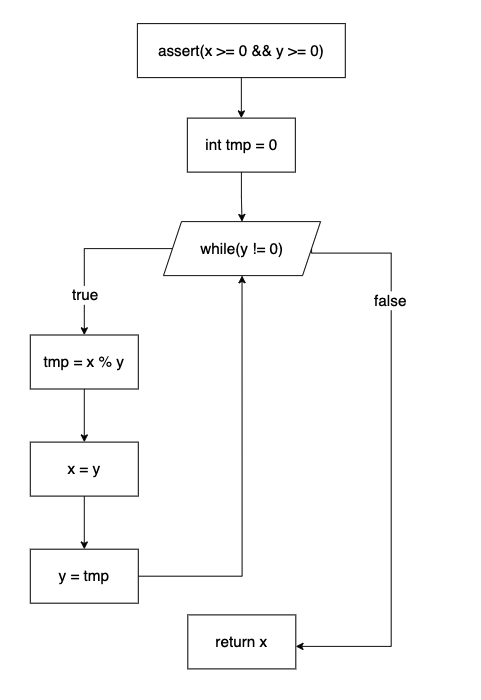
\includegraphics[width=250px]{6.10.1}

\subsubsection{Pregunta ii}
test1:
\begin{itemize}
    \item Entrada. $ x = 12, y = 8 $
    \item Salida esperada. $ 4 $
\end{itemize}

\subsection{Ejercicio 11}
\subsubsection{Pregunta i}
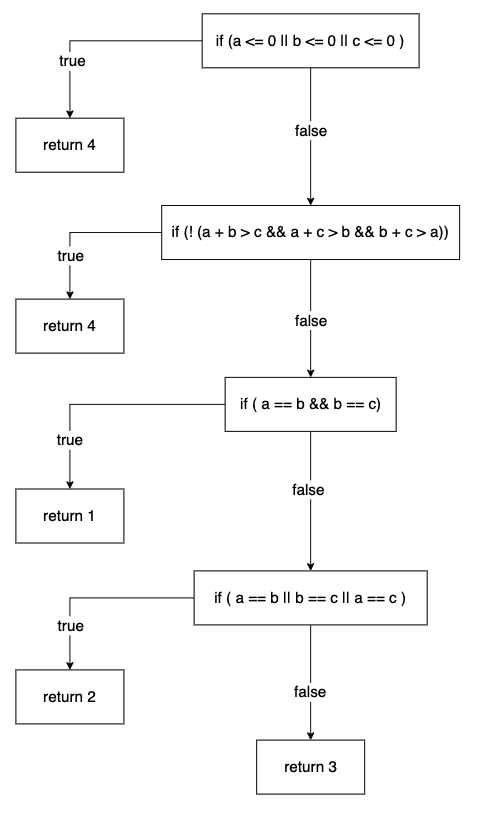
\includegraphics[width=250px]{6.11.1}

\subsubsection{Pregunta ii}
test1:
\begin{itemize}
    \item Entrada. $ a = -10, b = 2, c = 3 $
    \item Salida esperada. $ 4 $
\end{itemize}

test2:
\begin{itemize}
    \item Entrada. $ a = 1, b = 2, c = 4 $
    \item Salida esperada. $ 4 $
\end{itemize}

test3:
\begin{itemize}
    \item Entrada. $ a = 2, b = 2, c = 2 $
    \item Salida esperada. $ 1 $
\end{itemize}

test4:
\begin{itemize}
    \item Entrada. $ a = 2, b = 2, c = 3 $
    \item Salida esperada. $ 2 $
\end{itemize}

test5:
\begin{itemize}
    \item Entrada. $ a = 2, b = 3, c = 4 $
    \item Salida esperada. $ 3 $
\end{itemize}

El test suite (test1, test2, test3, test4, test5) ejecuta todas las lineas y todos los branches del programa.

\subsection{Ejercicio 12}
\subsubsection{Pregunta i}
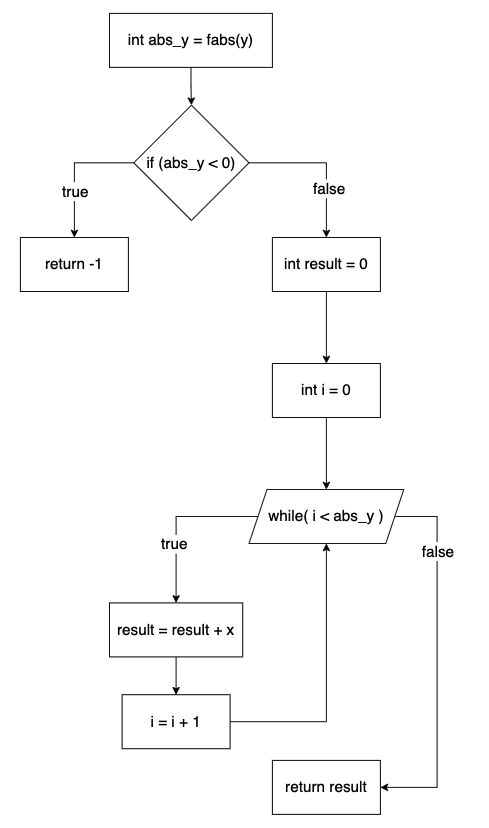
\includegraphics[width=250px]{6.12.1}

\subsubsection{Pregunta ii}
La rama true del primer if no puede ser cubierta por ningún caso de test pues la función fabs devuelve siempre un valor $ \geq 0 $

\subsubsection{Pregunta iii}
test1: 
\begin{itemize}
    \item Entrada. $ x = 2, y = -5 $
    \item Salida esperada. $ 10 $
\end{itemize}

test2: 
\begin{itemize}
    \item Entrada. $ x = 2, y = 0 $
    \item Salida esperada. $ 0 $
\end{itemize}

El segundo test lo agrego para ejecutar el falso de no ingreso al ciclo, aunque esa rama se cumpla siempre que se ingresa al ciclo.

\subsection{Ejercicio 13}
\subsubsection{Pregunta i}
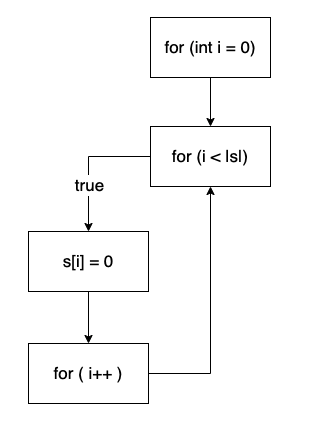
\includegraphics[width=200px]{6.13.1}

\subsubsection{Pregunta ii}
test1:
\begin{itemize}
    \item Entrada. $ s = \langle 1,2,3,4 \rangle $
    \item Salida esperada. $ \langle 0,0,0,0 \rangle $
\end{itemize}
Esto cubre todas las líneas del programa.

CONSULTAR que pasa con la lista vacía.

\subsubsection{Pregunta iii}
Si la lista vacía sigue la decisión del false del for, hay que agregarla como test.

\subsection{Ejercicio 14}
\subsubsection{Pregunta i}
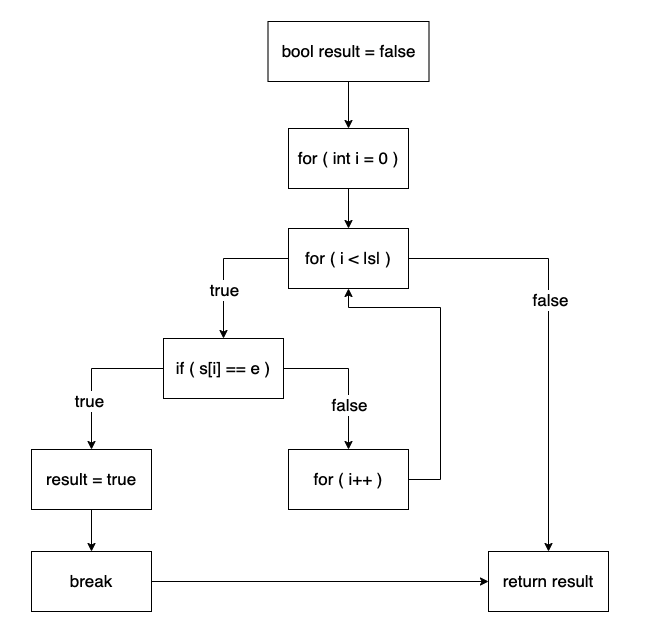
\includegraphics[width=300px]{6.14.1}

\subsubsection{Pregunta ii}
test1:
\begin{itemize}
    \item Entrada. $ s = \langle 1,2,3,4 \rangle; e = 3 $
    \item Salida esperada true
\end{itemize}

test2:
\begin{itemize}
    \item Entrada. $ s = \langle 1,2,3,4 \rangle; e = 5 $
    \item Salida esperada false
\end{itemize}
Cubre todas las lineas.

\subsubsection{Pregunta iii}
IDEM ejercicio anterior, agregar test de linea vacía si el no entrar al ciclo también es una decisión.

\subsection{Ejercicio 15}
\subsubsection{Pregunta i}
cantidadDePrimos

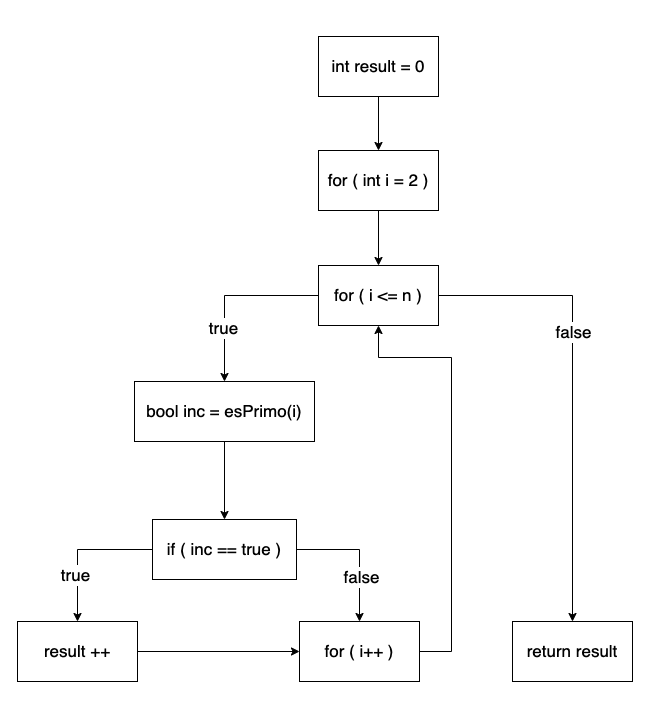
\includegraphics[width=300px]{6.15.1}

esPrimo

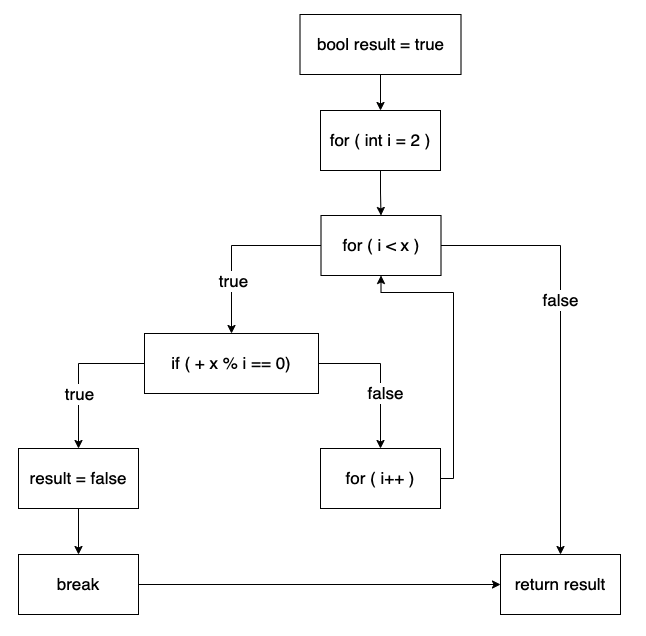
\includegraphics[width=300px]{6.15.2}

\subsubsection{Pregunta ii}
test1:
\begin{itemize}
    \item Entrada. $ n = 3 $
    \item Salida esperada $ 2 $
\end{itemize}

test2:
\begin{itemize}
    \item Entrada. $ n = 4 $
    \item Salida esperada $ 2 $
\end{itemize}
Cubre todas las líneas

\subsubsection{Pregunta iii}
En el video de la práctica agrega el test $ n = 0 $ que hace falsa la guarda del for.

\subsection{Ejercicio 16}
\subsubsection{Pregunta i}
esSubsecuencia

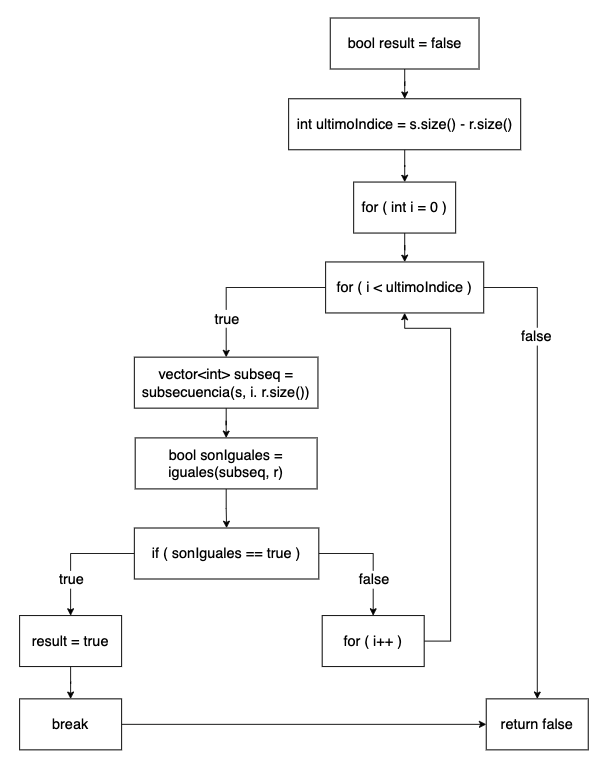
\includegraphics[width=300px]{6.16.1}

subsecuencia

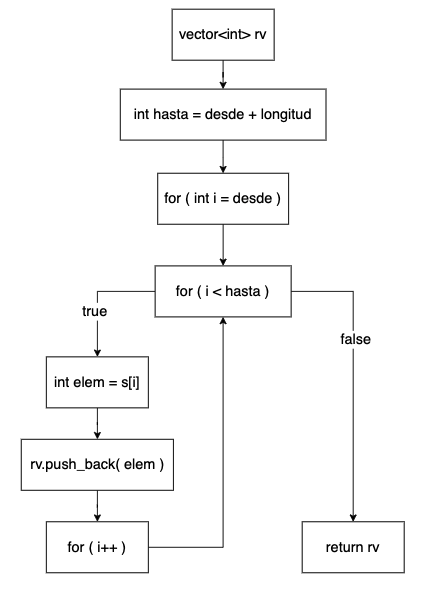
\includegraphics[width=250px]{6.16.2}

iguales

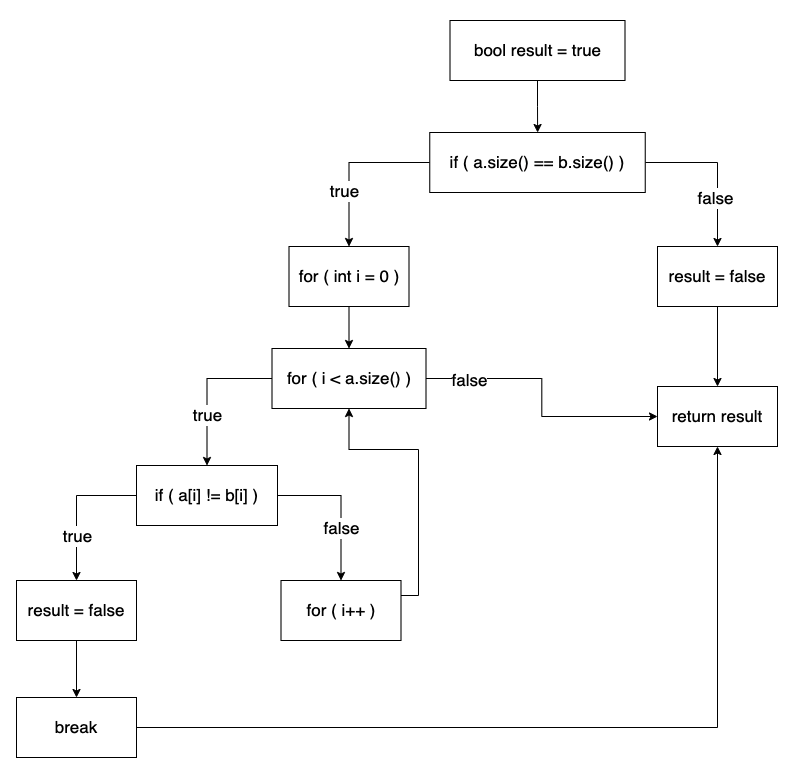
\includegraphics[width=300px]{6.16.3}

\subsubsection{Pregunta ii}
test1:
\begin{itemize}
    \item Entrada. $ s = \langle 1,2,3,4 \rangle; r = \langle 2,3 \rangle $
    \item Salida esperada true
\end{itemize}

test2:
\begin{itemize}
    \item Entrada. $ s = \langle 1,2 \rangle; r = \langle 1,2,3 \rangle $
    \item Salida esperada false
\end{itemize}

\end{document}
